\documentclass[ngerman]{scrartcl}
% Mögliche Sprachen: ngerman, USenglish, UKenglish

% \usepackage[utf8]{inputenc} % Ab TeX Live 2018 nicht mehr notwendig.
\usepackage[T1]{fontenc}
%\usepackage{babel}
\usepackage[autostyle=true]{csquotes}
\usepackage{mathtools}
\usepackage[ISO]{diffcoeff}
\usepackage{newtxtext}
\usepackage{newtxmath}
\usepackage{xfrac}
\usepackage{booktabs}  % Schönere Tabellen.
\usepackage{siunitx}   % Intelligentes Setzen von Zahlen und Einheiten.
\usepackage{hyperref}  % Klickbare Links.
\usepackage{placeins}
\usepackage{float}
\usepackage{enumitem}
\RequirePackage[backend=biber, style=numeric]{biblatex} %Literaturzitate
\addbibresource{file1.bib}

\KOMAoptions{fontsize=12pt,paper=a4}
\KOMAoptions{DIV=13}
\title{P4 Versuch 402 \\[1ex] \large Quantelung von Energie}
\author{Arieh Thill \& Noemi Ruppert}
\date{Mai 2025}
\begin{document}

\maketitle
\clearpage
\tableofcontents
\clearpage
%--------------------------------------------------------
\section{Einleitung}
Ein zentraler Versuch zur Bestätigung des Zusammenhangs zwischen der Quantelung von Energien und Emissions -und Absorptionslinien ist die Untersuchung des Photoeffekts. Die Spektroskopie ermöglicht die Untersuchung des Atomaufbaus, insbesondere durch die Analyse von Spektrallinien, welche einen Ausdruck der Quantelung von Energie sind und in direktem Zusammenhang mit Lichtfrequenzen stehen. \\
Im ersten Versuchsteil beobachtet man die Energieabhängigkeit des Photoeffekts und es werden das Planksche Wirkungsquantum, sowie die Austrittsarbeit abgeschätzt. 
\\
Im zweiten Versuchsteil wird durch Ausmeßung der Balmer-Linien das Planksche Wirkungsquantum erneut bestimmt und mit dem Ergebnis aus dem ersten Versuchsteil verglichen.
\clearpage
%--------------------------------------------------------
\section{Der Photo-Effekt}
\subsection{Grundlagen}
\subsubsection{Photoeffekt}
Der Photoeffekt tritt bei Ionisierung von Atomen durch Lichteinstrahlung, wobei die Energie der Valenzelektronen so weit ansteigt, dass sie das Potential des Atoms verlassen können. Dies geschieht nur, wenn das Licht eine Mindestenergie erreicht, die der Tiefe des Elektronenpotentials entspricht. Die Energie des Lichts \(E\) hängt mit ihrer Frequenz \(\nu\) durch die Beziehung \(E = \nu h\) zusammen, wobei \(h\) das Plancksche Wirkungsquantum darstellt. 
\subsubsection{Funktionsweise einer Photozelle}
\paragraph{Aufbau}
Eine Photozelle besteht aus einer Ringanode und einer Kathode, welche mit Licht beleuchtet
wird. Die Anode und die Kathode bestehen aus unterschiedlichen Materialien.


\begin{figure}[htbp]
    \centering
    \includegraphics[width=0.2\textwidth]{figs/anlegen_aeuß_potential.png}
    \caption{ Kontaktpotential $−eU_{KA}$ \cite{praktikum}}
    \label{fig:potential ext}
\end{figure}
\FloatBarrier

\begin{figure}[htbp]
    \centering
    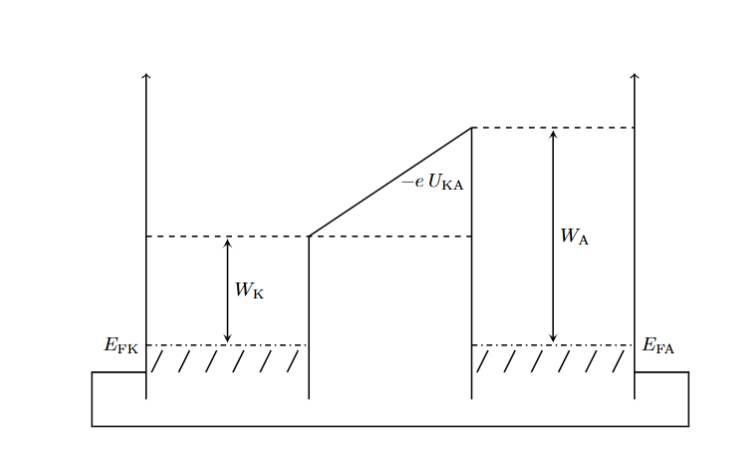
\includegraphics[width=0.2\textwidth]{figs/kontaktpotential_kurzgeschl_elektroden.png}
    \caption{  Potential dass von der Gegenspannung
$−eU_G$ induziert wird\cite{praktikum}}
    \label{fig:potential kurzg.}
\end{figure}
\FloatBarrier

\paragraph{Wirkung}
\begin{figure}[htbp]
    \centering
    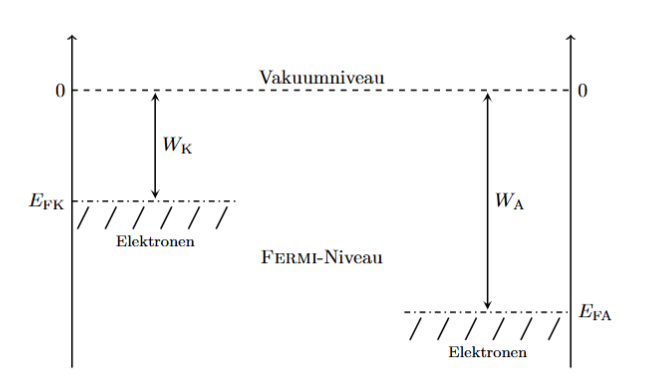
\includegraphics[width=0.2\textwidth]{figs/baenderschema_kathode_anode.png}
    \caption{ Ferminiveaus von Kathode und Anode mit Austrittsarbeit $W_A$ \cite{praktikum}}
    \label{fig:kathode-anode}
\end{figure}
\FloatBarrier
Das Anodenmaterial weist eine höhere Austrittsarbeit auf als das Kathodenmaterial, wodurch beim Kontakt eine Potentialdifferenz zwischen ihren Ferminiveaus entsteht. Diese Differenz verstärkt sich, wenn eine zusätzliche Gegenspannung zwischen Anode und Kathode angelegt wird.\\
Die durch das Licht herausgelösten Elektronen gewinnen entsprechend seiner Energie kinetische Energie und bewegen sich zur Anode, wodurch ein messbarer Strom entsteht. Die angelegte Gegenspannung verlangsamt die Elektronen und wird schrittweise erhöht, bis kein Photostrom mehr nachweisbar ist – also die Elektronen aus dem Anodenmaterial nicht mehr die Anode erreichen.
%\paragraph{Photostromverlauf}
%\paragraph{Austrittsarbeit}
%\paragraph{Kontaktpotential}

\subsection{Aufbau}
\begin{figure}[htbp]
    \centering
    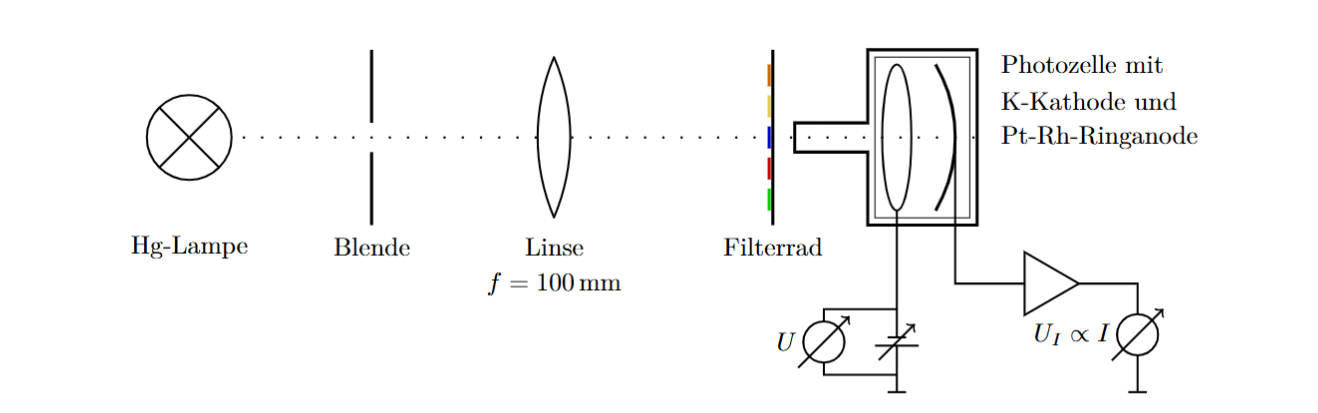
\includegraphics[width=0.5\textwidth]{figs/Aufbau_plank_wirkungsquantum.png}
    \caption{Aufbau für die Messung des Photoeffektes  \cite{praktikum}}
    \label{fig:aufbau teil 1}
\end{figure}
\FloatBarrier
Links ist die Hg-Lampe zu sehen, in der
Mitte Optik-Elemente zum Fokussieren und Filtern des Lichtes und rechts ist die Photozelle
mit Gegenspannung und Strommessung.

\subsection{Durchführung}
Die Quecksilber-Spektrallampe und die Photozelle werden gemäß Abbildung \ref{fig:aufbau teil 1} gegenüberliegend auf dem Reiter angeordnet. Eine Irisblende vor der Lampe ermöglicht die Regulierung der Lichtintensität. Eine Linse mit einer Brennweite von f=100 mm wird in diesem Abstand vor die Blende positioniert, sodass sie das Licht parallel auf den nachfolgenden Interferenzfilter mit fünf Filtern sowie eine zusätzliche Blende lenkt.\\
Eine Abschirmvorrichtung mit einem röhrenförmigen Element verhindert Streulicht. Ein Lichtfleck wird gezielt auf die Kathode projiziert, ohne ,dass die Anode beleuchtet wird. Der Anodenstrom wird über einen Messverstärker erfasst, während eine zum Strom proportionale Spannung mit einem Digitalmultimeter (DMM) gemessen wird. Die Gegenspannung stammt aus einem 12V-Gleichspannungsnetzteil, wobei der negative Pol mit der Anode verbunden ist, um die Elektronen abzubremsen. Diese Spannung wird mit einem weiteren DMM gemessen.
\subsection{Energiebilanz der Photoelektronen}
Laut der Abbildung der Ferminiveaus \ref{fig:kathode-anode} gilt für die Energiebilanz:
\begin{equation}
    E = h\nu = W_K + eU_{KA} + eU_{G,0} 
    = W_K + W_A - W_K + eU_{G,0} 
    = W_A + eU_{G,0}
\end{equation}\\
Aus der Frequenz des Lichtes können schließlich
die Austrittsarbeit der Anode $W_A$ und das Planck’sche Wirkungsquantum h bestimmt werden:
\begin{equation}
    eU_{G,0} = h\nu - W_A
\end{equation}
\subsection{Abschätzung des Plankschen Wirkungsquantum und der Austrittsarbeit}
\subsubsection{Bestimmung der Grenzspannung U_0}
\subsubsection{Bestimmung von Plankschen Wirkungsquantum h}
\subsubsection{Bestimmung der Austrittsarbeit W_A}
\subsubsection{Vergleich der $\lambda$ = Kennlinie für unterschiedliche Intensitäten }
%Diskussionen/Vergleiche werden direkt in den Unterteilen eingebaut
\clearpage
%--------------------------------------------------------
\section{Die Balmer-Serie}
\subsection{Grundlagen}
\subsubsection{Bohrsche Atommodel}
Im Bohrschen Atommodell bewegen sich die Elektronen auf bestimmten Kreisbahnen. Diese Kreisbahnen sind ein ganzzahliges Vielfaches der De Broglie Wellenlänge.
Wegen dem Kräftegleichgewichts zwischen Coulombkraft und Zentripetalkraft ergeben sich für die Radien der Kreisbahnen der Elektronen:
\begin{equation}
    r = \frac{n^2 h^2 \epsilon_0}{\pi \mu Z e^2} = \frac{n^2}{Z} a_0
\end{equation}\\
Wobei h das Plancksche Wirkungsquantum, $\mu$ die reduzierte Masse des Elektrons, Z die
Ladungsmenge, e die Elementarladung, n$\in \mathbf{N}$, $a_0$  der Bohrsche Radius ist.
\subsubsection{Balmer-Serie}
Elektronen können ihre Bahn wechseln, indem sie Energie in Form elektromagnetischer Wellen mit der Frequenz $\nu$ absorbieren oder emittieren, wobei ihre Energie durch $E = h\nu$ bestimmt wird. Die Lichtfrequenz während der Anregung oder Abregung eines Elektrons von einem Energieniveau zu einem Niveau folgt dem Zusammenhang:
\begin{equation}
    \nu = R_{\infty} c Z^2 \left( \frac{1}{n^2} - \frac{1}{m^2} \right)
\end{equation}\\
Dadurch wird die Energiedifferenz zwischen den beiden Zuständen mit Quantenzahlen n und m gegeben. Wobei $R_{\infty}$ der Rydberg-Konstante entspricht.\\
Für ein Wasserstoffatom gilt Z = 1 und mit n = 2 und $m> 2$ und man erhält die Balmerserie an Frequenzen die beobachtet werden und welche im sichtbaren Bereich sind.
\subsubsection{Quantenmechanische Betrachtung der Balmer-Serie}
\subsubsection{Isotopieaufspaltung}
Ein Isotop von Wasserstoff is Deuterum: sein Kern besteht aus einem Proton und einem extra Neutron.
Bei der Rydberg- Konstante muss dies berücksichtigt werden. Daraus folgt eine Verschiebung der Energie des emittierten Lichtstrahls. Bei diesen Kernen weißt sich der relative Massenunterschied besonders groß auf, wodurch die Verschiebung besonders deutlich sichtbar ist.
\subsubsection{Natürliche Linienbreite und Linienverbreiterungen}
\subsubsection{Reflexionsgitter}
\paragraph{Funktionsweise}
\paragraph{Auflösevermögen}

\subsection{Aufbau}

\subsection{Durchführung}

\subsection{Bestimmung der Gitterkonstanten}

\subsection{Bestimmung der Balmerlinien}
\subsubsection{Bestimmung der Isotopieaufspaltung}
\paragraph{Ermittelung des Peakschwerpunktes}
\paragraph{Ermittelung der Halbwertsbreite}
\subsubsection{Bestimmung der Rydberg-Konstante und des Plankschen Wirkungsquantum}
\paragraph{Rydberg-Konstante}
\paragraph{Planksche Wirkungsquantum}

\subsection{Weitergehende Überlegungen}
\subsubsection{Möglicher Ursprung der anderen auftrennen Spektrallinien}
\subsubsection{Doppler-Verbreitung}
\subsubsection{Auflösevermögen des Gitters}
\clearpage
%--------------------------------------------------------
\section{Fazit}

\clearpage
%--------------------------------------------------------
\section{Anhang}

\end{document}
